
%(BEGIN_QUESTION)

%Qualitatively graph the response of a proportional-plus-derivative controller over time to the following changes in process variable:

%$$\includegraphics[width=15.5cm]{i01540x01.eps}$$

%Assume {\it reverse} control action.

a) Kva er eit termoelement? Teikn skisse og forklår korleis det verkar. Kva temperaturområde kan vi måle med eit termoelement?
\\

\begin{tikzpicture}
	\draw[step=0.5cm,gray!20,very thin]  grid (15,10) ;
\end{tikzpicture}
\\
\eject
b) Forklar korleis eit pt-100 element er oppbygd og korleis det verkar. Teikn skisser og forklar korleis det vert kopla til ein måleomformar. Kvifor brukar vi helst tre-leder kopling mellom pt-100 elementet og måleomformaren.
\\

\begin{tikzpicture}
	\draw[step=0.5cm,gray!20,very thin]  grid (15,10) ;
\end{tikzpicture}
\\
c) Forklar uttrykka i måleteknikken: 
\begin{enumerate}
\item Tidskonstanten
\item Øvre målegrense
\item Nedre målegrense
\item Måle område
\end{enumerate}


\begin{tikzpicture}
	\draw[step=0.5cm,gray!20,very thin]  grid (15,8) ;
\end{tikzpicture}
\\

d) Nemn minst 5 forskjellege måleprinsipp for nivå i ein behaldar, og forklar måleprinsippet med ultralyd. Kva fordel er der med radarprinsippet i staden for ultralyd? 
\\

\begin{tikzpicture}
	\draw[step=0.5cm,gray!20,very thin]  grid (15,10) ;
\end{tikzpicture}
\\
e) Teikn skisse av ei veiecelle basera på strekklapp prinsippet og forklår korleis den verkar. Når er det mest aktuelt å bruka veieceller til nivåmåling?
\\

\begin{tikzpicture}
	\draw[step=0.5cm,gray!20,very thin]  grid (15,8) ;
\end{tikzpicture}
\\
f) Teikn ei prinsippskisse for ei hydraulisk veiecelle. 
\\

\begin{tikzpicture}
	\draw[step=0.5cm,gray!20,very thin]  grid (15,8) ;
\end{tikzpicture}
\eject 
g) Nemn nokre måleomformarar for nivå med av/på utgang. Kva kan vi bruke dei til?
\\

\begin{tikzpicture}
	\draw[step=0.5cm,gray!20,very thin]  grid (15,8) ;
\end{tikzpicture}
\\
\vfil
\pagebreak
Jon
\pagebreak
%Vi skal prosjektera ei veieselle for lastebilar, og vil bruka 4 hydrauliske sylindrar (ein i kvart hjørne) for å finna vekta. Ramma bilane køyrer opp på veg 16000kg. Fullasta bil kan vega 60000kg. Vi vil bruka 210 bar som maksimalt trykk i systemet. Rekn ut kor store sylindrar (diameter) vi må ha dersom vi reknar med maksimalt 50% skeivlast mellom målepunkta. Kan vi ha eit felles trykk i systemet, eller må vi ha 4 ulike målingar?

                         
%Teikn prinsippskisse!

	
%I ein kranbom som vist på teikninga er pila DB ein hydraulisk sylinder som skal lyfte ei vekt på 10 tonn i A. Vi har eit trykk i hydraulikken på 200 kg/cm². Avstandane er: A-B =10m, B-C = 2m, og vinkel d er 30°. Kor stor diameter må stempelet i sylinderen ha?


%\vfil

%\underbar{file i00000}
%\eject
%(END_QUESTION)





%(BEGIN_ANSWER)


%(END_ANSWER)





%(BEGIN_NOTES)


%INDEX% Alarm, ???: (word or phrase here)
%INDEX% Basics, transmitter: input and output ranges
%INDEX% Basics, ???: (word or phrase here)
%INDEX% Career, ???: (word or phrase here)
%INDEX% Calibration, table: (word or phrase here)
%INDEX% Calibration, ???: (word or phrase here)
%INDEX% Certification exam: (word or phrase here)
%INDEX% Chemistry, ???: (word or phrase here)
%INDEX% Control, proportional: (word or phrase here)
%INDEX% Control, derivative: (word or phrase here)
%INDEX% Control, integral: (word or phrase here)
%INDEX% Control, process characteristics: (word or phrase here)
%INDEX% Control, proportional + derivative: (word or phrase here)
%INDEX% Control, proportional + integral: (word or phrase here)
%INDEX% Control, proportional + integral + derivative: (word or phrase here)
%INDEX% Control, PID tuning: (word or phrase here)
%INDEX% Control, strategies: (word or phrase here)
%INDEX% Control, ???: (word or phrase here)
%INDEX% Course organization, ???: (word or phrase here)
%INDEX% Data Acquisition, ???: (word or phrase here)
%INDEX% DCS, ???: (word or phrase here)
%INDEX% Documentation, P&ID: (word or phrase here)
%INDEX% Documentation, loop diagram: (word or phrase here)
%INDEX% Documentation, functional: (word or phrase here)
%INDEX% Documentation, ???: (word or phrase here)
%INDEX% Electronics review: (word or phrase here)
%INDEX% Fieldbus, ???: (word or phrase here)
%INDEX% Final Control Elements, valve: (word or phrase here)
%INDEX% Final Control Elements, motor: (word or phrase here)
%INDEX% Final Control Elements, pump: (word or phrase here)
%INDEX% Good practices, wiring: ???
%INDEX% Good practices, ???: ???
%INDEX% Lab exercise, ???
%INDEX% Mathematics, calculus: (word or phrase here)
%INDEX% Mathematics, probability: (word or phrase here)
%INDEX% Measurement, pressure: (word or phrase here)
%INDEX% Measurement, level: (word or phrase here)
%INDEX% Measurement, temperature: (word or phrase here)
%INDEX% Measurement, flow: (word or phrase here)
%INDEX% Measurement, analytical: (word or phrase here)
%INDEX% Measurement, ???: (word or phrase here)
%INDEX% Mechanics, pneumatic instrument: (word or phrase here)
%INDEX% Mechanics, ???: (word or phrase here)
%INDEX% Networking, ???: (word or phrase here)
%INDEX% Physics, units and conversions: (word or phrase here)
%INDEX% Physics, energy, work, power: (word or phrase here)
%INDEX% Physics, static fluids: (word or phrase here)
%INDEX% Physics, temperature: (word or phrase here)
%INDEX% Physics, dynamic fluids: (word or phrase here)
%INDEX% Physics, ???: (word or phrase here)
%INDEX% PLC, ???: (word or phrase here)
%INDEX% Relay, ???: (word or phrase here)
%INDEX% Safety, ???: (word or phrase here)
%INDEX% Switch, pressure: (word or phrase here)
%INDEX% Switch, level: (word or phrase here)
%INDEX% Switch, temperature: (word or phrase here)
%INDEX% Switch, flow: (word or phrase here)
%INDEX% Switch, ???: (word or phrase here)
%INDEX% Troubleshooting circuit, ???

%(END_NOTES)


